\documentclass[conference]{IEEEtran}
\usepackage[utf8]{inputenc}
\usepackage{amsmath,amssymb}
\usepackage{graphicx}
\usepackage{booktabs}
\usepackage{url}
\usepackage[hidelinks]{hyperref}
\usepackage{cite}
\usepackage{array}

\setlength{\textfloatsep}{7pt plus 1pt minus 2pt}
\setlength{\floatsep}{6pt plus 1pt minus 2pt}
\setlength{\intextsep}{6pt plus 1pt minus 2pt}
\setlength{\abovecaptionskip}{3pt}
\setlength{\belowcaptionskip}{-2pt}

\begin{document}

\title{Benchmarking Multi-View Tree-Level Oil Palm Bunch Counting Under a Fixed Detector}

\author{
  \IEEEauthorblockN{Author Names}
  \IEEEauthorblockA{Institution\\City, Country\\email@example.com}
}

\maketitle

\begin{abstract}
Black Bunch Census (BBC) supports oil palm harvest planning by estimating,
for every tree, how many fresh fruit bunches (FFB) sit in each operational
maturity class. Image-based BBC is difficult because a single tree is observed
from multiple side views: additional views reduce occlusion, but the same
physical bunch can appear in several images and inflate naive counts. Despite an
active literature on agricultural detection and counting, no benchmark to date
has separated detector error from tree-level counter error for this task. This
paper benchmarks multi-view tree-level FFB counting for B1, B2, B3, and B4
under two carefully isolated detection conditions. In the \textit{GT detection
setting}, counters receive ground-truth boxes and classes, removing detector
quality as a source of error. In the \textit{fixed-detector setting}, counters
receive cached YOLOv26-medium outputs, measuring the deployed
detector-plus-counter pipeline. The benchmark uses 953 trees, 3,992 side-view
images, four maturity classes, 4 to 8 views per tree, and a fixed 716/96/141
train/validation/test split. Under GT detection, ElasticNet reaches 98.05\%
Class $\pm$1 Acc and 92.20\% Tree $\pm$1 Acc. Under the fixed detector, the
best Ridge + $F_{\text{all}}$ pipeline reaches 77.48\% Class $\pm$1 Acc and
32.62\% Tree $\pm$1 Acc. Feature ablation closes only $\approx$1.4\,pp Class
$\pm$1 Acc over the F0 baseline, and changing the counter family does not
recover the gap either. The conclusion is direct: tree-level counting is near
ceiling when detections are accurate, and the remaining 20.57\,pp gap is a
detector-quality bottleneck, not a counter limitation.
\end{abstract}

\begin{IEEEkeywords}
Oil palm, fresh fruit bunch, black bunch census, multi-view counting, object
detection, YOLO, tree-level regression, agricultural computer vision.
\end{IEEEkeywords}

% ---------------------------------------------------------------------------
\section{Introduction}
% ---------------------------------------------------------------------------

Oil palm harvest planning is driven by Black Bunch Census (BBC), a field
practice in which counters estimate, for every tree, how many bunches belong to
each operational maturity class: typically B1 (ripe, harvest now), B2
(imminent), B3 (next cycle), and B4 (future inventory)~\cite{ref11}. The
decision-relevant signal is therefore not the total number of bunches on a
tree, but the four-dimensional count vector across maturity classes.
Image-based BBC must reproduce this per-class disaggregation rather than
collapse it into a single total.

Tree-level counting is geometrically harder than image-level
detection~\cite{ref12}. Bunches surround the full circumference of an oil
palm, so a single image misses bunches because of occlusion, viewing angle, or
overlapping fronds. Multi-view acquisition reduces missed bunches by
photographing a tree from four or eight side views, but the same physical bunch
then appears in several of those images. Fig.~\ref{fig:crossview} illustrates
the effect: one B3 bunch is visible, and would be detected, in three adjacent
side views of tree \texttt{DAMIMAS\_A21B\_0847}. A naive sum over per-image
detections therefore counts appearances, not bunch identities, and is biased
upward by roughly a factor of two on this dataset.

\begin{figure*}[!t]
  \centering
  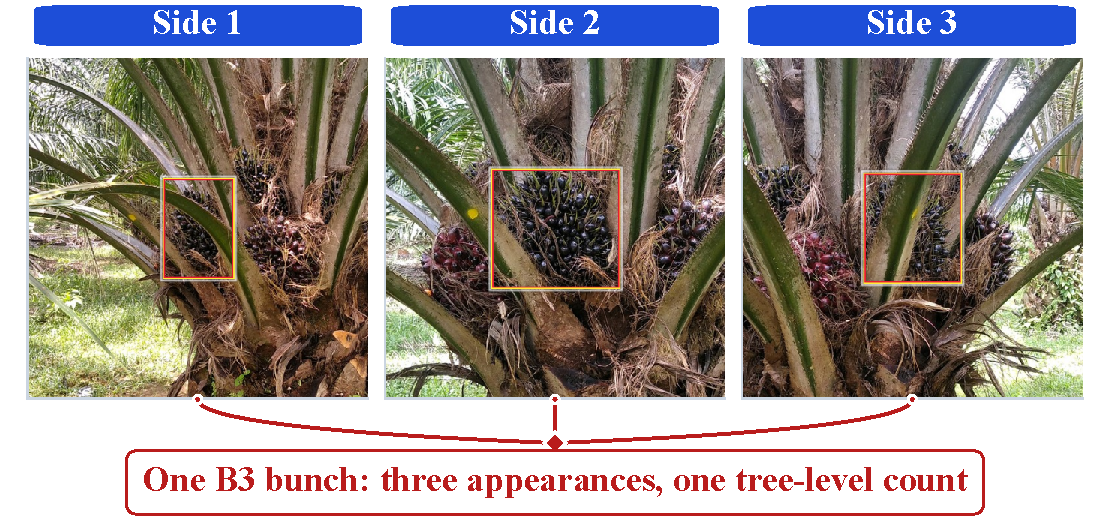
\includegraphics[width=\textwidth]{figures/paper/fig01_cross_view_linking.pdf}
  \caption{A single physical B3 bunch on tree \texttt{DAMIMAS\_A21B\_0847} is
  visible across sides 1, 2, and 3. If every per-image detection is counted,
  three appearances are added for one bunch. Tree-level counting must therefore
  aggregate evidence across views rather than sum it.}
  \label{fig:crossview}
\end{figure*}

Three lines of prior work bear on this problem. Oil palm FFB detection and
ripeness classification have been studied with both two-stage and YOLO-style
detectors~\cite{ref8,ref9,ref10,ref22}; these works show that detectors can
reach usable mAP on FFB but also document recurring weaknesses on partially
occluded or maturity-ambiguous bunches.

Multi-view fruit aggregation has been used in fruit recognition and yield
estimation, including methods that explicitly fuse evidence across views to
avoid double counting~\cite{ref5,ref6}. Comparative studies on apple orchards
and apple-and-orange counting from robotic platforms have further refined these
pipelines~\cite{ref14,ref15}. These methods, however, are evaluated mainly on
smaller tree-fruit crops with simpler geometry than oil palm, and they do not
isolate detector quality from aggregator quality.

Regression-based counting and yield estimation in agricultural vision are well
established~\cite{ref1,ref2,ref7,ref12,ref13}, and YOLO-style single-stage
detectors are now standard front-ends for such
pipelines~\cite{ref3,ref4,ref17,ref18}, with deep two-stage detectors also
widely applied in earlier orchard work~\cite{ref16}. In this line of work, a
regressor maps aggregate detection statistics to a target count, but the
regressor is typically evaluated only on the detector outputs at hand, leaving
the contribution of detector quality versus regressor quality unmeasured.

What is missing is a benchmark that determines, for tree-level multi-view BBC
counting, whether the limiting factor lies in the detector or in the tree-level
aggregator. Existing reports usually fix one component and tune the other,
conflating two error sources. This paper closes that gap. The contributions
are:
\begin{enumerate}
  \item \textbf{A systematic benchmark of tree-level bunch counting under two
    detection conditions.} Counter models are evaluated under GT detections
    (upper bound on counter performance) and under cached YOLOv26-medium
    outputs (deployed pipeline), with the same dataset split and the same
    evaluation metrics.
  \item \textbf{A feature ablation under realistic detector outputs.} Eight
    feature banks ranging from a 13-dimensional baseline to a 67-dimensional
    combined bank are evaluated with Ridge regression to identify which feature
    groups carry counting signal once detector noise is present.
  \item \textbf{Evidence that detector output quality is the primary
    bottleneck, not the counter.} The two settings differ by 20.57 percentage
    points in Class $\pm$1 Acc, and feature richness or counter choice closes
    only a small fraction of that gap.
\end{enumerate}

% ---------------------------------------------------------------------------
\section{Methodology}
% ---------------------------------------------------------------------------

\subsection{Dataset and Task Definition}

The benchmark uses the SawitMVC-YOLO multi-view dataset: 953 oil palm trees,
3,992 side-view images, four maturity classes (B1, B2, B3, and B4), and 4 to
8 side views per tree. The fixed split contains 716 training trees, 96
validation trees, and 141 test trees. Dataset construction, annotation
protocol, and per-class composition are documented in the companion dataset
release.

For tree $i$, the ground-truth target is the count vector
\begin{equation}
  \mathbf{y}_i = [\,y_{i,B1},\;y_{i,B2},\;y_{i,B3},\;y_{i,B4}\,],
\end{equation}
and the prediction is $\hat{\mathbf{y}}_i =
[\,\hat{y}_{i,B1},\ldots,\hat{y}_{i,B4}\,]$. The evaluation unit is the tree,
not the individual image: per-image appearance counts are not valid BBC outputs.

Let $a_{i,c}$ denote the number of detected appearances of class $c$ across
all views of tree $i$. The naive multi-view estimator
\begin{equation}
  \hat{y}_{i,c}^{\text{naive}} = a_{i,c}
\end{equation}
is biased upward whenever a bunch is visible from more than one side. Under GT
annotations, this estimator reaches only 50.00\% Class $\pm$1 Acc and 6.38\%
Tree $\pm$1 Acc on the test split, which motivates learned tree-level
aggregation rather than direct summation.

\subsection{Detection Conditions}

The benchmark isolates detector error from counter error by evaluating the same
counters under two detection conditions, illustrated in
Fig.~\ref{fig:conditions}.

\begin{figure}[!htbp]
  \centering
  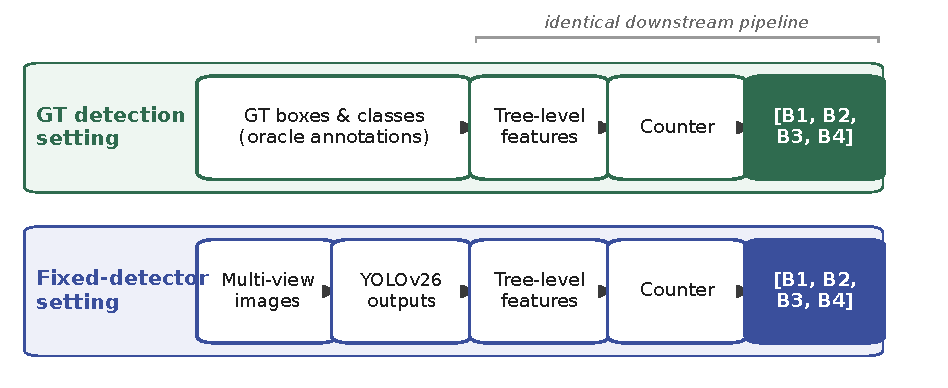
\includegraphics[width=\columnwidth]{figures/paper/fig02_detection_conditions.pdf}
  \caption{Two detection conditions used in the benchmark. \textit{Top:} the
  GT detection setting supplies ground-truth boxes and classes to the
  tree-level feature extractor, so detector output quality is removed as an
  error source. \textit{Bottom:} the fixed-detector setting supplies cached
  YOLOv26-medium outputs, so detector misses and class confusions enter the
  pipeline before counting.}
  \label{fig:conditions}
\end{figure}

In the \textit{GT detection setting}, the feature extractor reads ground-truth
bounding boxes and classes directly from the annotation files. Counters trained
on these features upper-bound how well a tree-level aggregator can perform when
detections are accurate. In the \textit{fixed-detector setting}, the feature
extractor reads cached YOLOv26-medium~\cite{ref18} predictions. A single
detector checkpoint is used for all counter and feature configurations so that
any observed differences are attributable to the counter or features, not to
detector retraining.

\begin{table}[!htbp]
  \centering
  \footnotesize
  \setlength{\tabcolsep}{4pt}
  \caption{YOLOv26-medium validation detection performance, reported under the
    COCO mAP50 convention~\cite{ref19}.}
  \label{tab:yolo}
  \begin{tabular}{@{}lrr@{}}
    \toprule
    Class   & mAP50          & Recall         \\
    \midrule
    B1      & \textbf{0.746} & \textbf{0.801} \\
    B2      & 0.425          & 0.433          \\
    B3      & 0.550          & 0.656          \\
    B4      & 0.363          & 0.389          \\
    Overall & 0.521          & 0.570          \\
    \bottomrule
  \end{tabular}
\end{table}

The detector is strongest on B1 and weakest on B4. The per-class weakness on
B4 and the moderate recall on B3 visible in Table~\ref{tab:yolo} are revisited
in Section~\ref{sec:gap}, where the per-class structure of the fixed-detector
gap mirrors this profile.

\subsection{Feature Vectors}

For each tree, detections from all views are aggregated into a fixed-length
feature vector. The 13-dimensional baseline F0 contains, for each class $c$,
the total count $s_c$, the per-side maximum $m_c$, and the per-side mean
$\mu_c$, plus the number of available views $n_{\text{views}}$:
\begin{equation}
  F0 = [\,s_{B1\text{:}B4},\;m_{B1\text{:}B4},\;\mu_{B1\text{:}B4},\;
        n_{\text{views}}\,].
\end{equation}

Three optional groups extend F0:
\begin{itemize}
  \item \textbf{Confidence (20-dim):} five statistics per class (confidence
    sum, mean, max, count above 0.5, and count above 0.6), summarizing how
    strongly detections are scored.
  \item \textbf{Spatial (8-dim):} two statistics per class (mean normalized
    vertical centroid $\overline{cy}_c$ and mean bounding-box area
    $\overline{A}_c$), capturing the fact that maturity classes tend to occupy
    distinct vertical zones on the tree.
  \item \textbf{Side-distribution (20-dim):} five statistics per class
    (per-side std, per-side min, coefficient of variation, number of sides with
    detections, and a consistency score), capturing how detections spread across
    the available views.
\end{itemize}

A cross-class composition group (6-dim), consisting of the total detection
count, four class fractions, and a B3-vs-(B2+B3) mixture ratio, completes the
67-dimensional combined bank $F_{\text{all}}$:
\begin{equation*}
  F_{\text{all}} = F0 \cup \text{conf} \cup \text{spatial}
                      \cup \text{distrib} \cup \text{composition}.
\end{equation*}

Eight feature banks are evaluated: F0, F0+conf, F0+spatial, F0+distrib,
F0+conf+spatial, F0+conf+distrib, F0+distrib+spatial, and $F_{\text{all}}$.

\subsection{Counter Models and Evaluation Metrics}

Five regression models are evaluated in both detection conditions: Linear
Regression, Ridge~\cite{ref23}, ElasticNet~\cite{ref20}, SVM~\cite{ref24}, and
Random Forest~\cite{ref21}. Each counter maps a tree feature vector
$\mathbf{x}_i$ to the count vector $\hat{\mathbf{y}}_i =
f_{\theta}(\mathbf{x}_i)$.

All counter models are trained on the 716-tree training split and evaluated on
the fixed 141-tree test split. Class-level $\pm 1$ correctness for tree $i$
and class $c$ is
\begin{equation}
  I_{i,c}^{\pm 1} =
  \begin{cases}
    1, & |\hat{y}_{i,c} - y_{i,c}| \leq 1, \\
    0, & \text{otherwise}.
  \end{cases}
\end{equation}

\textbf{Class $\pm$1 Acc} averages this indicator over all test trees and
classes:
\begin{equation}
  \text{Class } \pm 1 \text{ Acc} =
    \frac{1}{4N}\sum_{i=1}^{N}\sum_{c=1}^{4} I_{i,c}^{\pm 1}.
\end{equation}

\textbf{Tree $\pm$1 Acc} is stricter: a tree counts as correct only if all
four class predictions are within $\pm 1$ simultaneously,
\begin{equation}
  \text{Tree } \pm 1 \text{ Acc} =
    \frac{1}{N}\sum_{i=1}^{N}
      \mathbb{1}\!\left(\sum_{c=1}^{4} I_{i,c}^{\pm 1} = 4\right).
\end{equation}

\textbf{Macro MAE} is the mean absolute error averaged over trees and classes.
\textbf{Signed class bias} is the per-class mean $\hat{y}_{i,c} - y_{i,c}$;
positive values indicate over-counting, negative values under-counting. Bias
is reported alongside accuracy because operational aggregate yield estimates
are sensitive to directional error, not just absolute error.

% ---------------------------------------------------------------------------
\section{Results and Discussion}
% ---------------------------------------------------------------------------

The results are arranged to follow the argument: the ceiling first
(Section~\ref{sec:gt}), the reality under a real detector
(Section~\ref{sec:fixed}), the feature ablation that rules out the counter
side (Section~\ref{sec:ablation}), and the gap analysis that locates the
bottleneck (Section~\ref{sec:gap}).

\subsection{GT Detection Setting}
\label{sec:gt}

Table~\ref{tab:gt} reports counting results when the counter receives GT
detections. Naive appearance summation fails on the test set. This confirms
that duplicate visibility cannot be ignored. Both heuristic divisor rules
quickly recover to above 95\% Class $\pm$1 Acc, and learned counters push this
to 98.05\% with ElasticNet.

\begin{table}[!htbp]
  \centering
  \scriptsize
  \setlength{\tabcolsep}{2.3pt}
  \caption{Counting under the GT detection setting on the 141-tree test split.}
  \label{tab:gt}
  \begin{tabular}{@{}lcrrr@{}}
    \toprule
    Method                      & Type  & Class $\pm$1 & Tree $\pm$1 & MAE            \\
    \midrule
    Naive sum                   & Heur. & 50.00\%          &  6.38\%     & 2.142          \\
    Global divisor              & Heur. & 95.39\%          & 85.11\%     & 0.376          \\
    Visibility-adapt. divisor   & Heur. & 95.92\%          & 87.23\%     & 0.340          \\
    ElasticNet                  & ML    & \textbf{98.05\%} & \textbf{92.20\%} & 0.277      \\
    SVM                         & ML    & 97.87\%          & 91.49\%     & \textbf{0.266} \\
    Ridge                       & ML    & 97.70\%          & 90.78\%     & 0.275          \\
    Linear reg.                 & ML    & 97.52\%          & 90.07\%     & 0.277          \\
    Random forest               & ML    & 95.92\%          & 84.40\%     & 0.365          \\
    \bottomrule
  \end{tabular}
\end{table}

The four best machine-learning counters (ElasticNet, SVM, Ridge, LR) sit
within 0.5 percentage points of each other on Class $\pm$1 Acc and within 2.2
points on Tree $\pm$1 Acc; Random Forest is the only counter that
underperforms in this setting. The counter formulation, then, is not the
limiting factor: when detector evidence is accurate, simple regularized linear
models suffice to recover the BBC count.

\subsection{Fixed-Detector Setting}
\label{sec:fixed}

Table~\ref{tab:fixed} holds the feature bank at F0 and compares the five
counter families when they receive cached YOLOv26-medium outputs. The best F0
result, ElasticNet at 76.42\% Class $\pm$1 Acc, is more than 20 percentage
points below the ElasticNet result of the GT detection setting under the same
feature bank. All five counters fall within a 3.2 percentage-point window on
Class $\pm$1 Acc, reinforcing that the counter family is not what changed
between the two settings; only the detector did.

\begin{table}[!htbp]
  \centering
  \footnotesize
  \setlength{\tabcolsep}{3pt}
  \caption{Fixed-detector counting with F0 features on the 141-tree test split.}
  \label{tab:fixed}
  \begin{tabular}{@{}lrrr@{}}
    \toprule
    Counter           & Class $\pm$1 Acc & Tree $\pm$1 Acc  & Macro MAE      \\
    \midrule
    ElasticNet        & \textbf{76.42\%} & 29.79\%          & \textbf{1.043} \\
    Ridge             & 76.06\%          & 28.37\%          & 1.053          \\
    Linear Regression & 75.71\%          & \textbf{30.50\%} & 1.048          \\
    SVM               & 74.82\%          & 29.08\%          & \textbf{1.043} \\
    Random Forest     & 73.23\%          & 26.95\%          & 1.110          \\
    \bottomrule
  \end{tabular}
\end{table}

Per-class accuracies, listed in Table~\ref{tab:perclass}, reveal where the
loss concentrates: B1 stays above 95\% across all five counters, B2 sits
between 73.76\% and 80.14\%, and B3 collapses to between 55\% and 56\%. B4 is
intermediate, between 67\% and 73\%. This per-class profile mirrors the
per-class detector performance in Table~\ref{tab:yolo}, where B3 has moderate
recall and B4 has the lowest recall.

\begin{table}[!htbp]
  \centering
  \scriptsize
  \setlength{\tabcolsep}{3pt}
  \caption{Per-class Class $\pm$1 Acc of fixed-detector counters with F0
    features on the 141-tree test split.}
  \label{tab:perclass}
  \begin{tabular}{@{}lrrrr@{}}
    \toprule
    Counter           & B1               & B2               & B3               & B4               \\
    \midrule
    ElasticNet        & \textbf{96.45\%} & \textbf{80.14\%} & \textbf{56.03\%} & \textbf{73.05\%} \\
    Ridge             & 95.74\%          & \textbf{80.14\%} & \textbf{56.03\%} & 72.34\%          \\
    Linear Regression & \textbf{96.45\%} & 79.43\%          & 55.32\%          & 71.63\%          \\
    SVM               & 95.74\%          & 76.60\%          & 55.32\%          & 71.63\%          \\
    Random Forest     & 95.74\%          & 73.76\%          & \textbf{56.03\%} & 67.38\%          \\
    \bottomrule
  \end{tabular}
\end{table}

\subsection{Feature Ablation}
\label{sec:ablation}

\begin{table}[!htbp]
  \centering
  \scriptsize
  \setlength{\tabcolsep}{2.2pt}
  \caption{Ridge feature ablation in the fixed-detector setting.}
  \label{tab:ablation}
  \begin{tabular}{@{}>{\raggedright\arraybackslash}p{0.39\columnwidth}rrrr@{}}
    \toprule
    Features                            & Dim & Class $\pm$1 & Tree $\pm$1 & MAE            \\
    \midrule
    F0                                  &  13 & 76.06\%          & 28.37\%          & 1.053          \\
    F0 + confidence                     &  33 & 75.89\%          & 29.79\%          & 1.059          \\
    F0 + spatial                        &  21 & 76.60\%          & 30.50\%          & 1.046          \\
    F0 + side-distribution              &  33 & 74.82\%          & 28.37\%          & 1.060          \\
    F0 + confidence + spatial           &  41 & 76.24\%          & 29.08\%          & 1.059          \\
    F0 + confidence + side-distribution &  53 & 76.42\%          & 29.79\%          & 1.060          \\
    F0 + side-distribution + spatial    &  41 & 75.71\%          & 30.50\%          & 1.048          \\
    $F_{\text{all}}$                    &  67 & \textbf{77.48\%} & \textbf{32.62\%} & \textbf{1.035} \\
    \bottomrule
  \end{tabular}
\end{table}

Table~\ref{tab:ablation} holds the counter family fixed at Ridge (the strongest
counter under the richest feature bank) and varies only the feature
configuration. Spatial features alone bring 0.54 percentage points over F0,
confidence and side-distribution alone do not help, and the full $F_{\text{all}}$
bank reaches 77.48\% Class $\pm$1 Acc and 32.62\% Tree $\pm$1 Acc. The
headline absolute gain from F0 to $F_{\text{all}}$ is \textbf{+1.42 percentage
points} in Class $\pm$1 Acc and \textbf{+4.25 percentage points} in Tree
$\pm$1 Acc. This is the largest improvement that any feature ablation produces
in the fixed-detector setting, and it is small relative to the 20.57 percentage
points lost between the two settings. Feature engineering, therefore, can only
marginally compensate for what the detector did not supply.

\subsection{GT vs.\ Fixed-Detector Gap}
\label{sec:gap}

Fig.~\ref{fig:gap} visualises the central comparison. The top panel shows
per-class Class $\pm$1 Acc under both detection conditions; the bottom panel
shows the per-class signed bias of the best fixed-detector configuration.

\begin{figure}[!htbp]
  \centering
  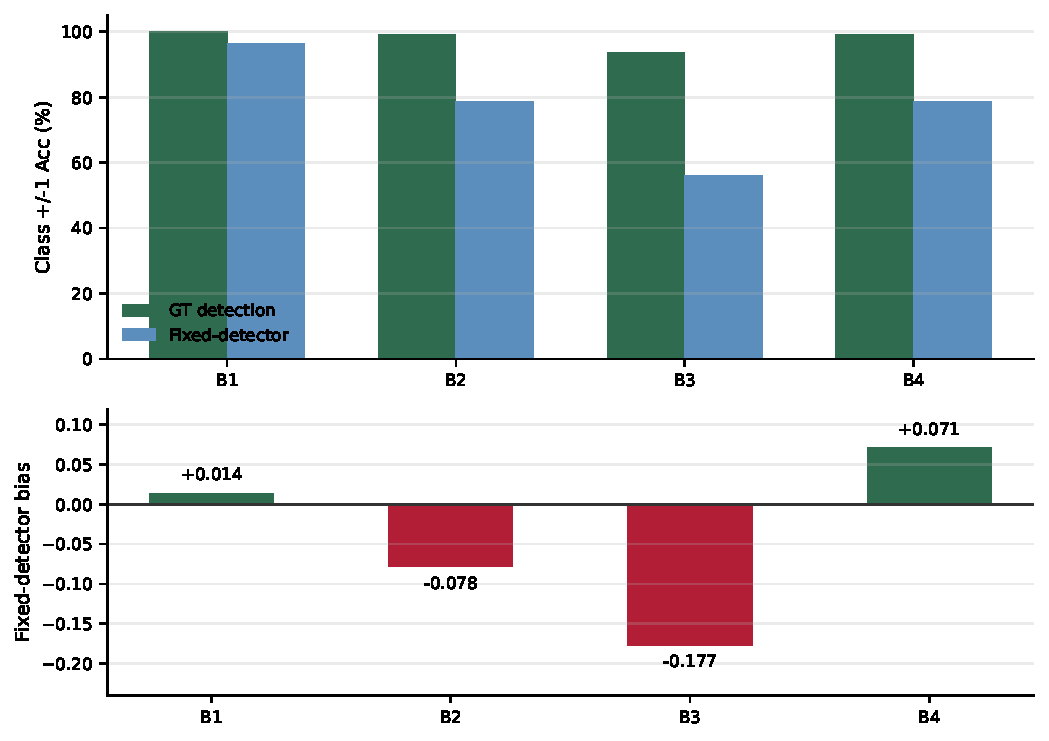
\includegraphics[width=\columnwidth]{figures/paper/fig03_gap_bias.pdf}
  \caption{\textit{Top:} Per-class Class $\pm$1 Acc for the best counter in
  each detection condition (ElasticNet under GT; Ridge + $F_{\text{all}}$ under
  the fixed detector). Counting is near ceiling under GT detection but drops
  sharply under the fixed detector. \textit{Bottom:} Per-class signed bias of
  Ridge + $F_{\text{all}}$ in the fixed-detector setting. Negative values
  indicate systematic under-counting; the under-count is concentrated on B2
  and especially B3.}
  \label{fig:gap}
\end{figure}

Three features of Fig.~\ref{fig:gap} stand out. The absolute gap is large, at
20.57 percentage points in Class $\pm$1 Acc and 59.58 percentage points in
Tree $\pm$1 Acc, summarised in Table~\ref{tab:summary}. Beyond its magnitude,
the gap has per-class structure. B1 loses only $\approx$2.8\,pp between the
two conditions, B2 loses $\approx$16.3\,pp, B3 loses 36.2\,pp, and B4 loses
$\approx$27.0\,pp. This profile aligns with the per-class detector performance
in Table~\ref{tab:yolo}, where the classes with weaker recall (B3, B4) fall
furthest below the GT ceiling. The bias is directional. The fixed-detector
Ridge + $F_{\text{all}}$ pipeline under-counts B2 by 0.078 and B3 by 0.177
bunches per tree on average. Because plantation-level yield estimates aggregate
per-tree predictions across blocks, a systematic per-class undercount in B2
and B3 propagates into a systematic underestimate of the next-cycle harvest
pipeline.

\begin{table}[!htbp]
  \centering
  \scriptsize
  \setlength{\tabcolsep}{2.4pt}
  \caption{Consolidated test-set summary. Biases are ordered by class.}
  \label{tab:summary}
  \begin{tabular}{@{}>{\raggedright\arraybackslash}p{0.27\columnwidth}rrrrrr@{}}
    \toprule
    Config & Class $\pm$1 & Tree $\pm$1 & B1 & B2 & B3 & B4 \\
    \midrule
    GT, ElasticNet &
      98.05\% & 92.20\% & $-.050$ & $+.043$ & $-.064$ & $-.028$ \\
    Fixed, Ridge + $F_{\text{all}}$ &
      77.48\% & 32.62\% & $+.014$ & $-.078$ & $-.177$ & $+.071$ \\
    \bottomrule
  \end{tabular}
\end{table}

Read together, Tables~\ref{tab:yolo}--\ref{tab:summary} with
Fig.~\ref{fig:gap} support a single interpretation. Multi-view duplicate
visibility is real and large, but it is well handled by learned tree-level
aggregation when detector evidence is accurate (Section~\ref{sec:gt}). Once a
fixed real-world detector replaces ground-truth boxes, counter performance
collapses (Section~\ref{sec:fixed}), and richer features or different counter
families recover only a small fraction of the loss
(Section~\ref{sec:ablation}). The per-class structure of the gap and of the
bias (Section~\ref{sec:gap} and Fig.~\ref{fig:gap}) is consistent with a
detector-quality bottleneck rather than a counter limitation.

Several limitations bound the scope of these findings. The benchmark uses a
single dataset of 953 trees from two plantations in South Kalimantan, so
absolute numbers may shift on other regions, varieties, or acquisition
protocols. Only one detector checkpoint (YOLOv26-medium) is evaluated, and a
different detector family could change the per-class error profile even if the
headline gap remains. The tree-level counters treat each tree independently and
ignore plantation-scale spatial or temporal regularities that operational
forecasts sometimes exploit. Finally, the four-class B1 through B4 taxonomy
admits visual ambiguity at the B2/B3 and B3/B4 boundaries, which places a soft
cap on what any detector-plus-counter pipeline can ultimately achieve.

Future work should therefore prioritize improving detector recall on B3 and B4,
calibrating detection confidence for counting use, and using explicit
cross-view association or geometry-aware aggregation rather than expanding the
tree-level feature bank further.

% ---------------------------------------------------------------------------
\section{Conclusion}
% ---------------------------------------------------------------------------

This paper benchmarks multi-view tree-level oil palm FFB counting under a
fixed detector by evaluating the same counters in a GT detection setting and a
fixed-detector setting. Under GT detection, ElasticNet reaches 98.05\% Class
$\pm$1 Acc and 92.20\% Tree $\pm$1 Acc on the 141-tree test split, showing
that the tree-level counter is near ceiling when detections are accurate. Under
the fixed YOLOv26-medium detector, the best Ridge + $F_{\text{all}}$ pipeline
reaches 77.48\% Class $\pm$1 Acc and 32.62\% Tree $\pm$1 Acc, and an
eight-bank feature ablation closes only $\approx$1.4 percentage points of the
gap. The remaining 20.57 percentage-point Class $\pm$1 Acc gap is therefore a
detector-quality bottleneck, not a counter limitation. The path to better
BBC-style B1 to B4 counting on this dataset runs primarily through better
detection, especially on B3 and B4, and through multi-view evidence handling
that is explicitly designed around detector uncertainty.

% ---------------------------------------------------------------------------
\section*{Acknowledgment}
% ---------------------------------------------------------------------------

To be completed with institutional, funding, plantation-access, and
data-collection acknowledgments before submission.

% ---------------------------------------------------------------------------
\section*{Code and Data Availability}
% ---------------------------------------------------------------------------

Code: \url{https://github.com/ULM-SawitMVC/Baseline-SawitMVC}

Data: \url{https://huggingface.co/datasets/ULM-DS-Lab/SawitMVC-YOLO}

% ---------------------------------------------------------------------------
\begin{thebibliography}{24}

\bibitem{ref1}
A.~Koirala, K.~B.~Walsh, Z.~Wang, and C.~McCarthy,
``Deep learning: method overview and review of use for fruit detection and
yield estimation,''
\textit{Computers and Electronics in Agriculture}, vol.~162, pp.~219--234,
Jul.~2019, doi: \url{10.1016/j.compag.2019.04.017}.

\bibitem{ref2}
A.~Kamilaris and F.~X.~Prenafeta-Bold\'{u},
``Deep learning in agriculture: A survey,''
\textit{Computers and Electronics in Agriculture}, vol.~147, pp.~70--90,
Apr.~2018, doi: \url{10.1016/j.compag.2018.02.016}.

\bibitem{ref3}
J.~Redmon, S.~Divvala, R.~Girshick, and A.~Farhadi,
``You Only Look Once: Unified, real-time object detection,''
in \textit{Proc. IEEE Conf. Computer Vision and Pattern Recognition (CVPR)},
2016, pp.~779--788, doi: \url{10.1109/CVPR.2016.91}.

\bibitem{ref4}
A.~Bochkovskiy, C.-Y.~Wang, and H.-Y.~M.~Liao,
``YOLOv4: Optimal speed and accuracy of object detection,''
arXiv:2004.10934, 2020.

\bibitem{ref5}
Y.~Song, C.~A.~Glasbey, G.~W.~Horgan, G.~Polder, and
G.~W.~A.~M.~van~der~Heijden,
``Automatic fruit recognition and counting from multiple images,''
\textit{Biosystems Engineering}, vol.~118, pp.~203--215, Feb.~2014,
doi: \url{10.1016/j.biosystemseng.2013.12.008}.

\bibitem{ref6}
M.~Stein, S.~Bargoti, and J.~Underwood,
``Image based mango fruit detection, localisation and yield estimation using
multiple view geometry,''
\textit{Sensors}, vol.~16, no.~11, Art. no.~1915, Nov.~2016,
doi: \url{10.3390/s16111915}.

\bibitem{ref7}
I.~Sa, Z.~Ge, F.~Dayoub, B.~Upcroft, T.~Perez, and C.~McCool,
``DeepFruits: A fruit detection system using deep neural networks,''
\textit{Sensors}, vol.~16, no.~8, Art. no.~1222, Aug.~2016,
doi: \url{10.3390/s16081222}.

\bibitem{ref8}
N.~A.~Prasetyo, Pranowo, and A.~J.~Santoso,
``Automatic detection and calculation of palm oil fresh fruit bunches using
Faster R-CNN,''
\textit{International Journal of Applied Science and Engineering}, vol.~17,
no.~2, pp.~121--134, 2020, doi: \url{10.6703/IJASE.202005_17(2).121}.

\bibitem{ref9}
J.~W.~Lai, H.~R.~Ramli, L.~I.~Ismail, and W.~Z.~W.~Hasan,
``Real-time detection of ripe oil palm fresh fruit bunch based on YOLOv4,''
\textit{IEEE Access}, vol.~10, pp.~95763--95770, 2022,
doi: \url{10.1109/ACCESS.2022.3204762}.

\bibitem{ref10}
M.~Y.~M.~A.~Mansour, K.~D.~Dambul, and K.~Y.~Choo,
``Object detection algorithms for ripeness classification of oil palm fresh
fruit bunch,''
\textit{International Journal of Technology}, vol.~13, no.~6,
pp.~1326--1335, 2022, doi: \url{10.14716/ijtech.v13i6.5932}.

\bibitem{ref11}
M.~Kerstan and T.~Fairhurst,
``Use of OMP for accurate crop forecasts,''
Agrisoft Systems and Tropical Crop Consultants Limited. [Online]. Available:
\url{https://www.agrisoft-systems.com/wp-content/uploads/Papers/CropForecastsWithOMPBBC.pdf}

\bibitem{ref12}
V.~Lempitsky and A.~Zisserman,
``Learning to count objects in images,''
in \textit{Proc. Advances in Neural Information Processing Systems (NeurIPS)},
2010, pp.~1324--1332.

\bibitem{ref13}
M.~Rahnemoonfar and C.~Sheppard,
``Deep count: Fruit counting based on deep simulated learning,''
\textit{Sensors}, vol.~17, no.~4, Art. no.~905, Apr.~2017,
doi: \url{10.3390/s17040905}.

\bibitem{ref14}
N.~H\"{a}ni, P.~Roy, and V.~Isler,
``A comparative study of fruit detection and counting methods for yield
mapping in apple orchards,''
\textit{Journal of Field Robotics}, vol.~37, no.~2, pp.~263--282, Mar.~2020,
doi: \url{10.1002/rob.21902}.

\bibitem{ref15}
S.~W.~Chen et al.,
``Counting apples and oranges with deep learning: A data-driven approach,''
\textit{IEEE Robotics and Automation Letters}, vol.~2, no.~2, pp.~781--788,
Apr.~2017, doi: \url{10.1109/LRA.2017.2651944}.

\bibitem{ref16}
S.~Bargoti and J.~Underwood,
``Deep fruit detection in orchards,''
in \textit{Proc. IEEE International Conference on Robotics and Automation
(ICRA)}, 2017, pp.~3626--3633, doi: \url{10.1109/ICRA.2017.7989417}.

\bibitem{ref17}
C.-Y.~Wang, A.~Bochkovskiy, and H.-Y.~M.~Liao,
``YOLOv7: Trainable bag-of-freebies sets new state-of-the-art for real-time
object detectors,''
in \textit{Proc. IEEE/CVF Conference on Computer Vision and Pattern
Recognition (CVPR)}, 2023, pp.~7464--7475,
doi: \url{10.1109/CVPR52729.2023.00721}.

\bibitem{ref18}
G.~Jocher, A.~Chaurasia, and J.~Qiu,
``Ultralytics YOLO,'' 2023. [Online]. Available:
\url{https://github.com/ultralytics/ultralytics}

\bibitem{ref19}
T.-Y.~Lin et al.,
``Microsoft COCO: Common objects in context,''
in \textit{Proc. European Conference on Computer Vision (ECCV)}, 2014,
pp.~740--755, doi: \url{10.1007/978-3-319-10602-1_48}.

\bibitem{ref20}
H.~Zou and T.~Hastie,
``Regularization and variable selection via the elastic net,''
\textit{Journal of the Royal Statistical Society B}, vol.~67, no.~2,
pp.~301--320, 2005, doi: \url{10.1111/j.1467-9868.2005.00503.x}.

\bibitem{ref21}
L.~Breiman,
``Random forests,''
\textit{Machine Learning}, vol.~45, no.~1, pp.~5--32, 2001,
doi: \url{10.1023/A:1010933404324}.

\bibitem{ref22}
M.~H.~Junos, A.~S.~M.~Khairuddin, S.~Thannirmalai, and M.~Dahari,
``Automatic detection of oil palm fruits from UAV images using an improved
YOLO model,''
\textit{The Visual Computer}, vol.~38, no.~7, pp.~2341--2355, 2022,
doi: \url{10.1007/s00371-021-02116-3}.

\bibitem{ref23}
A.~E.~Hoerl and R.~W.~Kennard,
``Ridge regression: Biased estimation for nonorthogonal problems,''
\textit{Technometrics}, vol.~12, no.~1, pp.~55--67, 1970,
doi: \url{10.1080/00401706.1970.10488634}.

\bibitem{ref24}
C.~Cortes and V.~Vapnik,
``Support-vector networks,''
\textit{Machine Learning}, vol.~20, no.~3, pp.~273--297, 1995,
doi: \url{10.1007/BF00994018}.

\end{thebibliography}

\end{document}
